% ============================================================
%  SESSION 2 — Modern JavaScript
%  XeLaTeX ile derleyin: xelatex session-02.tex
% ============================================================
\documentclass[12pt, a4paper]{article}

% ---------- Font & Dil ----------
\usepackage{fontspec}
\usepackage[turkish, shorthands=off]{babel}
\setmainfont{Georgia}
\setsansfont{Arial}
\setmonofont{Courier New}

% ---------- Sayfa Düzeni ----------
\usepackage[top=2.2cm, bottom=2.2cm, left=2.4cm, right=2.4cm]{geometry}
\usepackage{parskip}
\setlength{\parindent}{0pt}

% ---------- Renkler ----------
\usepackage{xcolor}
\definecolor{primary}{HTML}{2563EB}
\definecolor{secondary}{HTML}{7C3AED}
\definecolor{accent}{HTML}{059669}
\definecolor{warning}{HTML}{D97706}
\definecolor{danger}{HTML}{DC2626}
\definecolor{lightbg}{HTML}{F1F5F9}
\definecolor{codebg}{HTML}{1E293B}
\definecolor{codefg}{HTML}{E2E8F0}
\definecolor{jscol}{HTML}{F7DF1E}
\definecolor{jskw}{HTML}{93C5FD}
\definecolor{jsstr}{HTML}{86EFAC}
\definecolor{jscomment}{HTML}{94A3B8}
\definecolor{jsfn}{HTML}{FCA5A5}
\definecolor{promisecol}{HTML}{F59E0B}
\definecolor{asynccol}{HTML}{8B5CF6}

% ---------- Kutular (tcolorbox) ----------
\usepackage[skins, breakable, listings]{tcolorbox}
\tcbuselibrary{skins, breakable, listings}

\newtcolorbox{infobox}[1][]{
  enhanced, breakable,
  colback=primary!8, colframe=primary,
  fonttitle=\bfseries\sffamily,
  title={#1},
  left=6pt, right=6pt, top=4pt, bottom=4pt,
  arc=4pt
}

\newtcolorbox{warningbox}[1][]{
  enhanced, breakable,
  colback=warning!10, colframe=warning,
  fonttitle=\bfseries\sffamily,
  title={#1},
  left=6pt, right=6pt, top=4pt, bottom=4pt,
  arc=4pt
}

\newtcolorbox{practicebox}[1][]{
  enhanced, breakable,
  colback=accent!8, colframe=accent,
  fonttitle=\bfseries\sffamily,
  title={#1},
  left=6pt, right=6pt, top=4pt, bottom=4pt,
  arc=4pt
}

\newtcolorbox{definebox}[1][]{
  enhanced, breakable,
  colback=secondary!7, colframe=secondary,
  fonttitle=\bfseries\sffamily,
  title={#1},
  left=6pt, right=6pt, top=4pt, bottom=4pt,
  arc=4pt
}

\newtcolorbox{dangerbox}[1][]{
  enhanced, breakable,
  colback=danger!7, colframe=danger,
  fonttitle=\bfseries\sffamily,
  title={#1},
  left=6pt, right=6pt, top=4pt, bottom=4pt,
  arc=4pt
}

% ---------- Kod Listeleme ----------
\usepackage{listings}

\lstset{literate=
  {ı}{{\texttt{i}}}1  {İ}{{\texttt{I}}}1
  {ğ}{{\texttt{g}}}1  {Ğ}{{\texttt{G}}}1
  {ş}{{\texttt{s}}}1  {Ş}{{\texttt{S}}}1
  {ü}{{\texttt{u}}}1  {Ü}{{\texttt{U}}}1
  {ö}{{\texttt{o}}}1  {Ö}{{\texttt{O}}}1
  {ç}{{\texttt{c}}}1  {Ç}{{\texttt{C}}}1
}

\lstdefinestyle{jsstyle}{
  backgroundcolor=\color{codebg},
  basicstyle=\ttfamily\small\color{codefg},
  keywordstyle=\color{jskw}\bfseries,
  stringstyle=\color{jsstr},
  commentstyle=\color{jscomment}\itshape,
  morekeywords={let, const, var, async, await, of, from, import, export,
    default, class, extends, new, return, true, false, null, undefined,
    function, arrow, Promise, fetch, then, catch, finally, try,
    map, filter, reduce, forEach, find, findIndex, some, every,
    console, log, JSON, stringify, parse},
  morestring=[b]",
  morestring=[b]',
  morestring=[b]`,
  morecomment=[l]{//},
  morecomment=[s]{/*}{*/},
  showstringspaces=false,
  breaklines=true,
  frame=none,
  xleftmargin=8pt, xrightmargin=8pt,
}

% ---------- Grafikler ----------
\usepackage{graphicx}
\usepackage{caption}
\usepackage{tikz}
\usetikzlibrary{arrows.meta, shapes.geometric, positioning, calc}

% ---------- Tablo ----------
\usepackage{booktabs}
\usepackage{tabularx}
\usepackage{array}

% ---------- Başlık Stilleri ----------
\makeatletter
\renewcommand{\section}{%
  \@startsection{section}{1}{\z@}%
    {-1.5ex plus -1ex minus -0.5ex}%
    {0.8ex plus 0.3ex}%
    {\normalfont\Large\bfseries\sffamily\color{primary}}%
}
\renewcommand{\subsection}{%
  \@startsection{subsection}{2}{\z@}%
    {-1.2ex plus -0.8ex minus -0.4ex}%
    {0.5ex plus 0.2ex}%
    {\normalfont\large\bfseries\sffamily\color{secondary}}%
}
\renewcommand{\subsubsection}{%
  \@startsection{subsubsection}{3}{\z@}%
    {-1ex plus -0.6ex minus -0.3ex}%
    {0.4ex}%
    {\normalfont\normalsize\bfseries\sffamily\color{accent}}%
}
\makeatother

% ---------- Üstbilgi / Altbilgi ----------
\usepackage{fancyhdr}
\setlength{\headheight}{14pt}
\pagestyle{fancy}
\fancyhf{}
\fancyhead[L]{\small\sffamily\color{gray} Front-end + Next.js Eğitimi}
\fancyhead[R]{\small\sffamily\color{gray} Session 2 --- Modern JavaScript}
\fancyfoot[C]{\small\sffamily\color{gray} \thepage}
\renewcommand{\headrulewidth}{0.4pt}

% ---------- Diğer ----------
\usepackage{enumitem}
\setlist[itemize]{leftmargin=1.5em, itemsep=2pt}
\setlist[enumerate]{leftmargin=1.5em, itemsep=2pt}
\usepackage{hyperref}
\hypersetup{colorlinks=true, linkcolor=primary, urlcolor=primary}
\usepackage{fontawesome5}

% ---------- Yardımcı Komut ----------
\newcommand{\timebadge}[1]{%
  \noindent
  \colorbox{primary}{\color{white}\sffamily\bfseries\small\strut~~\faStopwatch~~#1~~}%
  \par\vspace{4pt}%
}

\newcommand{\jsinline}[1]{\texttt{\color{primary}#1}}

% ============================================================
\begin{document}

% ============================================================
%  KAPAK
% ============================================================
\thispagestyle{empty}

\begin{tikzpicture}[remember picture, overlay]
  \fill[primary] (current page.north west)
    rectangle ++(\paperwidth, -8.0cm);
  \fill[secondary] (current page.north west) ++(0,-7.8cm)
    rectangle ++(\paperwidth, -0.28cm);
\end{tikzpicture}

\vspace*{1.6cm}
{\color{white}\sffamily
  \hspace{1.2cm}{\small SESSION 2 / 8 \quad|\quad 29 Nisan 2026 \quad|\quad~90 dakika}\\[12pt]
  \hspace{1.2cm}{\fontsize{30}{36}\selectfont\bfseries Modern JavaScript}\\[8pt]
  \hspace{1.2cm}{\Large React Öncesi Gerekli JS Bilgisi}
}

\vspace{0.9cm}

\vspace{0.1cm}

\begin{tcolorbox}[enhanced,
  colback=lightbg, colframe=gray!30, arc=4pt,
  title={\sffamily\bfseries\color{primary}\faStream\quad Session Akışı},
  fonttitle=\bfseries\sffamily]
\sffamily\small
\begin{tabularx}{\textwidth}{>{\bfseries\color{primary}}l X l}
\toprule
Süre & Konu & Anahtar Kavramlar \\
\midrule
0--20 dk  & Değişkenler ve Fonksiyonlar    & let/const, arrow function, template literal \\
20--50 dk & Veri Dönüştürme                & destructuring, spread/rest, map/filter/reduce \\
50--75 dk & Asenkron JavaScript            & Promise, async/await, fetch API \\
75--90 dk & \textcolor{accent}{Pratik: API'den liste çek} & fetch + render \\
\bottomrule
\end{tabularx}
\end{tcolorbox}

% ============================================================
\clearpage
\section{\faJs\ Değişkenler ve Modern Fonksiyonlar}
\timebadge{0--20 dakika}

\subsection{var, let, const Farkı}

JavaScript'te değişken tanımlamak için üç anahtar kelime vardır.
Modern kodda \texttt{var} \textbf{kullanılmaz}; \texttt{let} ve \texttt{const} tercih edilir.

\vspace{8pt}

\begin{tcolorbox}[enhanced, colback=codebg, colframe=gray!30,
    colbacktitle=primary!85!black, coltitle=white, arc=4pt,
    title={\sffamily\bfseries\small var vs let vs const}]
\begin{lstlisting}[style=jsstyle]
// var — avoid, can cause problems
var name = "Ahmet";
var name = "Mehmet"; // redeclaration: no error (bad)

// let — mutable value
let score = 0;
score = 10;       // OK

// const — constant binding (for primitives the value is constant)
const PI = 3.14;
// PI = 3;       // ERROR: const cannot be reassigned

// const with object/array: binding is constant, contents can change
const user = { name: "Ali", age: 30 };
user.age = 31;  // OK — content changed
// user = {};   // ERROR — binding cannot change
\end{lstlisting}
\end{tcolorbox}

\vspace{6pt}

\begin{tcolorbox}[enhanced, colback=lightbg, colframe=gray!30, arc=4pt]
\sffamily\small
\begin{tabularx}{\textwidth}{>{\ttfamily\bfseries\color{primary}}l X X X}
\toprule
\normalfont\bfseries & \normalfont\bfseries Yeniden atama & \normalfont\bfseries Yeniden tanımlama & \normalfont\bfseries Kapsam \\
\midrule
var   & Evet & Evet & Fonksiyon \\
let   & Evet & Hayır & Blok (\{ \}) \\
const & Hayır & Hayır & Blok (\{ \}) \\
\bottomrule
\end{tabularx}
\end{tcolorbox}

\begin{warningbox}[\faLightbulb\ Altın Kural]
\textbf{Önce \texttt{const} dene.} Değer değişmesi gerekiyorsa \texttt{let} kullan.
\texttt{var}'a hiç gerek yok.
\end{warningbox}

% ----------------------------------------------------------
\subsection{Arrow Functions (Ok Fonksiyonları)}

Arrow function, fonksiyon yazmanın daha kısa yoludur.
React'ta her yerde karşımıza çıkacak.

\vspace{6pt}

\begin{tcolorbox}[enhanced, colback=codebg, colframe=gray!30,
    colbacktitle=primary!85!black, coltitle=white, arc=4pt,
    title={\sffamily\bfseries\small Normal vs Arrow Function}]
\begin{lstlisting}[style=jsstyle]
// --- Normal function ---
function sum(a, b) {
  return a + b;
}

// --- Arrow function (equivalent) ---
const sum = (a, b) => {
  return a + b;
};

// --- Short form: single expression => no {} and no return ---
const sum = (a, b) => a + b;

// --- Single parameter: parentheses optional ---
const square = x => x * x;

// --- No parameters ---
const greet = () => "Hello!";

// Usage
console.log(sum(3, 5));   // 8
console.log(square(4));   // 16
console.log(greet());     // "Hello!"
\end{lstlisting}
\end{tcolorbox}

\vspace{6pt}

\begin{infobox}[\faLightbulb\ Ne Zaman Kullanılır?]
React'ta component tanımlarında, event handler'larda ve
\texttt{map/filter} gibi callback'lerde arrow function kullanmak
standart haline gelmiştir.
\end{infobox}

% ----------------------------------------------------------
\subsection{Template Literals (Şablon Dizeler)}

Değişken birleşimi için \texttt{+} yerine daha okunaklı bir yöntem.

\vspace{6pt}

\begin{tcolorbox}[enhanced, colback=codebg, colframe=gray!30,
    colbacktitle=primary!85!black, coltitle=white, arc=4pt,
    title={\sffamily\bfseries\small Template Literal Örneği}]
\begin{lstlisting}[style=jsstyle]
const name = "Zeynep";
const age  = 28;

// Old way — harder to read
const message1 = "Hello, " + name + "! Your age: " + age;

// Template literal — written with backticks (` )
const message2 = `Hello, ${name}! Your age: ${age}`;

// You can use expressions too
const message3 = `${age >= 18 ? "Adult" : "Minor"}: ${name}`;

// Multiline text
const html = `
  <div>
    <h1>${name}</h1>
    <p>Age: ${age}</p>
  </div>
`;
\end{lstlisting}
\end{tcolorbox}

% ============================================================
\newpage
\section{\faTools\ Veri Dönüştürme Araçları}
\timebadge{20--50 dakika}

\subsection{Destructuring (Parçalama)}

Nesne veya diziden değerleri tek satırda çıkarmak için kullanılır.
React'ta \textbf{props} ve \textbf{state} kullanımı buna dayanır.

\vspace{6pt}

\begin{tcolorbox}[enhanced, colback=codebg, colframe=gray!30,
    colbacktitle=primary!85!black, coltitle=white, arc=4pt,
    title={\sffamily\bfseries\small Object Destructuring}]
\begin{lstlisting}[style=jsstyle]
const user = {
  name: "Can",
  age: 25,
  city: "Istanbul"
};

// Old way
const name  = user.name;
const age   = user.age;

// With destructuring
const { name, age } = user;

// Renaming
const { name: firstName, age: yearsOld } = user;
console.log(firstName);          // "Can"

// Default value
const { country = "Turkey" } = user;
console.log(country);        // "Turkey" (not present in object)

// In function parameters — React props often look like this
function UserCard({ name, age }) {
  return `${name} (${age})`;
}
\end{lstlisting}
\end{tcolorbox}

\vspace{6pt}

\begin{tcolorbox}[enhanced, colback=codebg, colframe=gray!30,
    colbacktitle=primary!85!black, coltitle=white, arc=4pt,
    title={\sffamily\bfseries\small Array Destructuring}]
\begin{lstlisting}[style=jsstyle]
const colors = ["red", "green", "blue"];

// Destructuring
const [first, second] = colors;
console.log(first); // "red"
console.log(second);  // "green"

// Skipping
const [, , third] = colors;
console.log(third);  // "blue"

// React useState uses this exact format:
const [count, setCount] = useState(0);
//      ^value  ^updater
\end{lstlisting}
\end{tcolorbox}

% ----------------------------------------------------------
\subsection{Spread ve Rest Operatörleri (\texttt{...})}

Üç nokta (\texttt{...}) iki farklı işlem için kullanılır:
\textbf{spread} (yaymak) ve \textbf{rest} (toplamak).

\vspace{6pt}

\begin{tcolorbox}[enhanced, colback=codebg, colframe=gray!30,
    colbacktitle=primary!85!black, coltitle=white, arc=4pt,
    title={\sffamily\bfseries\small Spread — Dizi ve Nesne Birleştirme}]
\begin{lstlisting}[style=jsstyle]
// Dizi spread
const a = [1, 2, 3];
const b = [4, 5, 6];
const all = [...a, ...b];       // [1, 2, 3, 4, 5, 6]
const copy  = [...a];            // does not affect original

// Object spread — React state updates often look like this
const user = { name: "Ali", age: 30 };
const updated    = { ...user, age: 31 };
// { name: "Ali", age: 31 }

// Fonksiyon cagrilarinda
const numbers = [3, 1, 4, 1, 5];
console.log(Math.max(...numbers)); // 5
\end{lstlisting}
\end{tcolorbox}

\vspace{6pt}

\begin{tcolorbox}[enhanced, colback=codebg, colframe=gray!30,
    colbacktitle=primary!85!black, coltitle=white, arc=4pt,
    title={\sffamily\bfseries\small Rest — Kalan Parametreleri Topla}]
\begin{lstlisting}[style=jsstyle]
// Fonksiyon parametrelerinde rest
function sum(...numbers) {
  return numbers.reduce((acc, n) => acc + n, 0);
}
console.log(sum(1, 2, 3, 4)); // 10

// Rest in destructuring
const [first, second, ...rest] = [10, 20, 30, 40, 50];
console.log(first);      // 10
console.log(rest); // [30, 40, 50]

const { name, ...otherInfo } = user;
// otherInfo = { age: 30 }
\end{lstlisting}
\end{tcolorbox}

% ----------------------------------------------------------
\newpage
\subsection{Array Methods — map, filter, reduce}

\begin{definebox}[Neden Önemli?]
React'ta liste render etmek için \texttt{map}, veri filtrelemek için
\texttt{filter} kullanılır. Bu metotlar orijinal diziyi \textbf{değiştirmez},
\textbf{yeni dizi döndürür}.
\end{definebox}

\vspace{8pt}

\subsubsection{map — Her Elemanı Dönüştür}

\begin{tcolorbox}[enhanced, colback=codebg, colframe=gray!30,
    colbacktitle=primary!85!black, coltitle=white, arc=4pt,
    title={\sffamily\bfseries\small map Örnekleri}]
\begin{lstlisting}[style=jsstyle]
const numbers = [1, 2, 3, 4, 5];

// Square each number
const squares = numbers.map(n => n * n);
// [1, 4, 9, 16, 25]

// Transform an array of objects
const users = [
  { id: 1, name: "Ali" },
  { id: 2, name: "Veli" },
];

const names = users.map(u => u.name);
// ["Ali", "Veli"]

// In React: create a list of elements
// users.map(u => <li key={u.id}>{u.name}</li>)
\end{lstlisting}
\end{tcolorbox}

\vspace{6pt}

\subsubsection{filter — Koşulu Sağlayanları Al}

\begin{tcolorbox}[enhanced, colback=codebg, colframe=gray!30,
    colbacktitle=primary!85!black, coltitle=white, arc=4pt,
    title={\sffamily\bfseries\small filter Örnekleri}]
\begin{lstlisting}[style=jsstyle]
const products = [
  { name: "Pencil",   price: 5,   inStock: true  },
  { name: "Notebook", price: 15,  inStock: false },
  { name: "Eraser",   price: 3,   inStock: true  },
  { name: "Ruler",    price: 8,   inStock: true  },
];

// In-stock products
const inStock = products.filter(p => p.inStock === true);
// [{Pencil}, {Eraser}, {Ruler}]

// Products cheaper than 10
const cheapOnes = products.filter(p => p.price < 10);
// [{Pencil}, {Eraser}, {Ruler}]

// Search filter example
const query = "pe";
const results = products.filter(p =>
  p.name.toLowerCase().includes(query)
);
// [{Pencil}]
\end{lstlisting}
\end{tcolorbox}

\vspace{6pt}

\subsubsection{reduce — Tek Değere İndir (Yüzeysel)}

\begin{tcolorbox}[enhanced, colback=codebg, colframe=gray!30,
    colbacktitle=primary!85!black, coltitle=white, arc=4pt,
    title={\sffamily\bfseries\small reduce Örneği}]
\begin{lstlisting}[style=jsstyle]
const prices = [10, 25, 8, 42, 15];

// Toplam hesapla
const total = prices.reduce((acc, price) => acc + price, 0);
//                               ^birikim  ^su anki eleman   ^baslangic
console.log(total); // 100

// Nesne dizisinde toplam
const cart = [
  { product: "Pencil",   quantity: 3, price: 5  },
  { product: "Notebook", quantity: 1, price: 15 },
];

const totalAmount = cart.reduce(
  (acc, item) => acc + (item.quantity * item.price),
  0
);
console.log(totalAmount); // 30
\end{lstlisting}
\end{tcolorbox}

\vspace{8pt}

% Görsel: map/filter/reduce akışı
\begin{center}
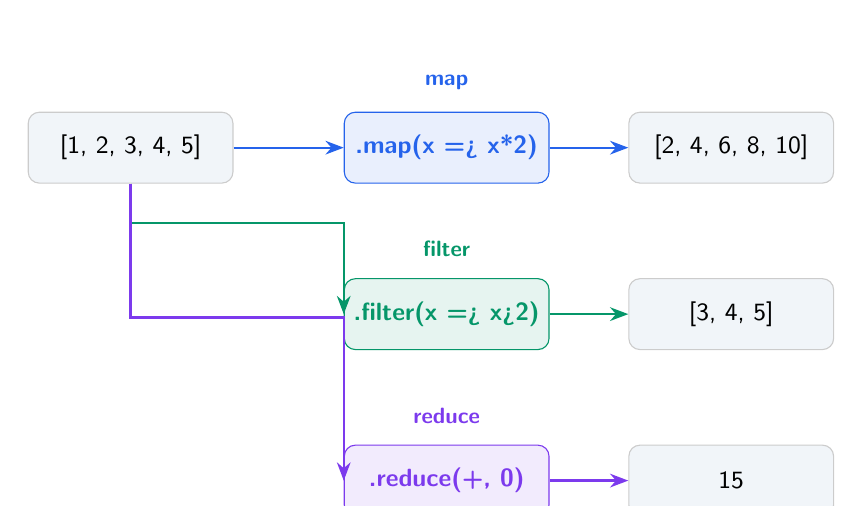
\begin{tikzpicture}[node distance=1.0cm, >=Stealth]

  % Orijinal dizi
  \node[draw=gray!40, fill=lightbg, rounded corners=4pt,
        minimum width=2.6cm, minimum height=0.9cm,
        font=\sffamily\small] (arr)
        {[1, 2, 3, 4, 5]};

  % map
  \node[draw=primary, fill=primary!10, rounded corners=4pt,
        minimum width=2.6cm, minimum height=0.9cm,
        font=\sffamily\small\bfseries\color{primary},
        right=1.4cm of arr] (mapnode)
        {.map(x => x*2)};

  \node[draw=gray!40, fill=lightbg, rounded corners=4pt,
        minimum width=2.6cm, minimum height=0.9cm,
        font=\sffamily\small,
        right=1.0cm of mapnode] (mapout)
        {[2, 4, 6, 8, 10]};

  \draw[->, thick, primary] (arr) -- node[above, font=\sffamily\tiny]{} (mapnode);
  \draw[->, thick, primary] (mapnode) -- (mapout);
  \node[font=\sffamily\footnotesize\bfseries\color{primary}, above=0.15cm of mapnode] {map};

  % filter
  \node[draw=accent, fill=accent!10, rounded corners=4pt,
        minimum width=2.6cm, minimum height=0.9cm,
        font=\sffamily\small\bfseries\color{accent},
        below=1.2cm of mapnode] (filternode)
        {.filter(x => x>2)};

  \node[draw=gray!40, fill=lightbg, rounded corners=4pt,
        minimum width=2.6cm, minimum height=0.9cm,
        font=\sffamily\small,
        right=1.0cm of filternode] (filterout)
        {[3, 4, 5]};

  \draw[->, thick, accent] (arr.south) -- ++(0,-0.5) -| (filternode.west);
  \draw[->, thick, accent] (filternode) -- (filterout);
  \node[font=\sffamily\footnotesize\bfseries\color{accent}, above=0.15cm of filternode] {filter};

  % reduce
  \node[draw=secondary, fill=secondary!10, rounded corners=4pt,
        minimum width=2.6cm, minimum height=0.9cm,
        font=\sffamily\small\bfseries\color{secondary},
        below=1.2cm of filternode] (reducenode)
        {.reduce(+, 0)};

  \node[draw=gray!40, fill=lightbg, rounded corners=4pt,
        minimum width=2.6cm, minimum height=0.9cm,
        font=\sffamily\small,
        right=1.0cm of reducenode] (reduceout)
        {15};

  \draw[->, thick, secondary] (arr.south) -- ++(0,-1.7) -| (reducenode.west);
  \draw[->, thick, secondary] (reducenode) -- (reduceout);
  \node[font=\sffamily\footnotesize\bfseries\color{secondary}, above=0.15cm of reducenode] {reduce};

\end{tikzpicture}
\end{center}

% ============================================================
\newpage
\section{\faClock\ Asenkron JavaScript}
\timebadge{50--75 dakika}

\subsection{Neden Asenkron?}

JavaScript \textbf{tek thread}'lidir: bir işlem bitene kadar diğer işlemler bekler.
API'den veri çekme, dosya okuma gibi işlemler zaman alır.
Bunları \textbf{asenkron} yaparak kullanıcı arayüzü donup kalmasını önleriz.

\vspace{8pt}

\begin{center}
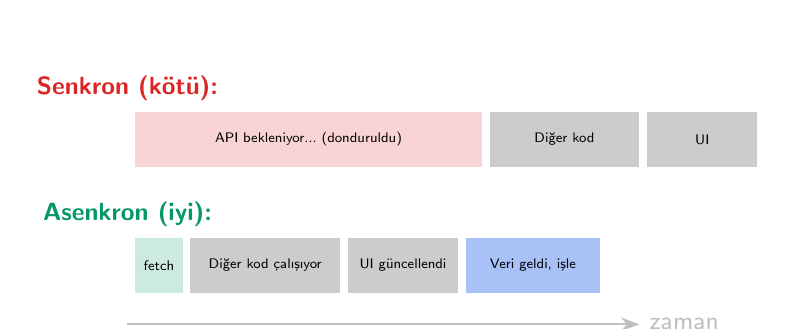
\begin{tikzpicture}[node distance=0.5cm, >=Stealth]

  % Senkron timeline
  \node[font=\sffamily\bfseries\small, text=danger] at (0, 4.2) {Senkron (kötü):};
  \fill[danger!20] (0.1,3.2) rectangle (4.5,3.9);
  \fill[gray!40]   (4.6,3.2) rectangle (6.5,3.9);
  \fill[gray!40]   (6.6,3.2) rectangle (8.0,3.9);
  \node[font=\sffamily\tiny] at (2.3, 3.55) {API bekleniyor... (donduruldu)};
  \node[font=\sffamily\tiny] at (5.55,3.55) {Diğer kod};
  \node[font=\sffamily\tiny] at (7.3, 3.55) {UI};

  % Asenkron timeline
  \node[font=\sffamily\bfseries\small, text=accent] at (0, 2.6) {Asenkron (iyi):};
  \fill[accent!20] (0.1,1.6) rectangle (0.7,2.3);
  \fill[gray!40]   (0.8,1.6) rectangle (2.7,2.3);
  \fill[gray!40]   (2.8,1.6) rectangle (4.2,2.3);
  \fill[primary!40](4.3,1.6) rectangle (6.0,2.3);
  \node[font=\sffamily\tiny] at (0.4, 1.95) {fetch};
  \node[font=\sffamily\tiny] at (1.75,1.95) {Diğer kod çalışıyor};
  \node[font=\sffamily\tiny] at (3.5, 1.95) {UI güncellendi};
  \node[font=\sffamily\tiny] at (5.15,1.95) {Veri geldi, işle};

  % Zaman oku
  \draw[->, thick, gray!50] (0.0, 1.2) -- (6.5, 1.2)
    node[right, font=\sffamily\small] {zaman};

\end{tikzpicture}
\end{center}

% ----------------------------------------------------------
\subsection{Promise}

\texttt{Promise}, \textit{``şu an elimde yok ama geldiğinde sana vereyim''} sözü veren bir nesnedir.

\vspace{6pt}

\begin{tcolorbox}[enhanced, colback=codebg, colframe=gray!30,
    colbacktitle=promisecol!85!black, coltitle=white, arc=4pt,
    title={\sffamily\bfseries\small Promise Mantığı}]
\begin{lstlisting}[style=jsstyle]
// Promise has 3 states: pending -> fulfilled | rejected
const promise = new Promise((resolve, reject) => {
  const success = true;

  if (success) {
    resolve("Data arrived!");  // fulfilled
  } else {
    reject("An error occurred!");  // rejected
  }
});

// Listen for the result
promise
  .then(data  => console.log(data))   // "Data arrived!"
  .catch(err => console.error(err));

// fetch() returns a Promise:
fetch("https://api.example.com/users")
  .then(response => response.json())  // convert to JSON
  .then(data     => console.log(data))
  .catch(err     => console.error(err));
\end{lstlisting}
\end{tcolorbox}

\vspace{6pt}

% ----------------------------------------------------------
\subsection{async / await}

\texttt{async/await}, Promise'leri \textbf{sanki senkronmuş gibi} yazmanın yoludur.
Okunması ve hata yakalaması çok daha kolaydır.

\vspace{6pt}

\begin{tcolorbox}[enhanced, colback=codebg, colframe=gray!30,
    colbacktitle=asynccol!85!black, coltitle=white, arc=4pt,
    title={\sffamily\bfseries\small async/await --- Temel Kullanım}]
\begin{lstlisting}[style=jsstyle]
// An \"async\" function returns a Promise
async function fetchUsers() {
  // \"await\" waits for a Promise without freezing the UI thread
  const response = await fetch(
    "https://jsonplaceholder.typicode.com/users"
  );

  // response.json() also returns a Promise
  const data = await response.json();

  return data;
}

// Error handling: try/catch
async function fetchSafely() {
  try {
    const response = await fetch("https://api.example.com/data");

    if (!response.ok) {
      throw new Error(`HTTP error: ${response.status}`);
    }

    const data = await response.json();
    console.log(data);
  } catch (err) {
    console.error("An error occurred:", err.message);
  }
}
\end{lstlisting}
\end{tcolorbox}

\vspace{6pt}

\begin{tcolorbox}[enhanced, colback=lightbg, colframe=gray!30, arc=4pt]
\sffamily\small
\begin{tabularx}{\textwidth}{X X}
\toprule
\bfseries .then().catch() & \bfseries async/await \\
\midrule
Zincir şeklinde yazılır & Düz sıra gibi okunur \\
Her adımda callback & try/catch ile hata yakalar \\
Bazı durumlarda daha kısa & Daha okunaklı, tercih edilir \\
\bottomrule
\end{tabularx}
\end{tcolorbox}

\vspace{6pt}

% ----------------------------------------------------------
\subsection{fetch API}

\texttt{fetch}, tarayıcının dahili HTTP istek fonksiyonudur.
Dış kütüphanesiz API çağrısı yapmak için kullanılır.

\vspace{6pt}

\begin{tcolorbox}[enhanced, colback=codebg, colframe=gray!30,
    colbacktitle=primary!85!black, coltitle=white, arc=4pt,
    title={\sffamily\bfseries\small fetch ile GET ve POST}]
\begin{lstlisting}[style=jsstyle]
// GET — veri cekme (en sik kullanilan)
async function postlariGetir() {
  const response = await fetch(
    "https://jsonplaceholder.typicode.com/posts"
  );
  const postlar = await response.json();
  return postlar; // dizi donuyor
}

// POST — veri gonderme
async function yeniPostOlustur(baslik, icerik) {
  const response = await fetch(
    "https://jsonplaceholder.typicode.com/posts",
    {
      method: "POST",
      headers: {
        "Content-Type": "application/json",
      },
      body: JSON.stringify({ baslik, icerik }),
    }
  );
  const yeniPost = await response.json();
  console.log("Olusturuldu:", yeniPost);
}
\end{lstlisting}
\end{tcolorbox}

\begin{infobox}[\faLink\ Pratikte Kullanacağımız API]
\textbf{JSONPlaceholder} --- \texttt{https://jsonplaceholder.typicode.com}\\
Ücretsiz, kayıt gerektirmeyen sahte (fake) REST API.
\texttt{/posts}, \texttt{/users}, \texttt{/todos} endpoint'leri var.
\end{infobox}

% ============================================================
\newpage
\section{\faHammer\ Pratik: API'den Veri Çekme ve Liste Render}
\timebadge{75--90 dakika}

\begin{practicebox}[\faTasks\ Pratik Hedef]
JSONPlaceholder API'sinden kullanıcı listesi çek ve sayfada listele.
\begin{itemize}
  \item \texttt{fetch} ile \texttt{GET /users} isteği at
  \item Gelen kullanıcıları \texttt{map} ile HTML'e dönüştür
  \item Sayfaya enjekte et
\end{itemize}
\end{practicebox}

\vspace{8pt}
\textbf{Adım 1 --- HTML Yapısı}

\begin{tcolorbox}[enhanced, colback=codebg, colframe=gray!30,
    colbacktitle=primary!85!black, coltitle=white, arc=4pt,
    title={\sffamily\bfseries\small index.html}]
\begin{lstlisting}[style=jsstyle]
<!DOCTYPE html>
<html lang="tr">
<head>
  <meta charset="UTF-8" />
  <title>User List</title>
  <link rel="stylesheet" href="style.css" />
</head>
<body>
  <header>
    <h1>Users</h1>
  </header>

  <main>
    <!-- JS will render cards here -->
    <div id="user-list">
      <p>Loading...</p>
    </div>
  </main>

  <!-- Script at the end -->
  <script src="app.js"></script>
</body>
</html>
\end{lstlisting}
\end{tcolorbox}

\vspace{8pt}
\textbf{Adım 2 --- JavaScript (app.js)}

\begin{tcolorbox}[enhanced, colback=codebg, colframe=gray!30,
    colbacktitle=primary!85!black, coltitle=white, arc=4pt,
    title={\sffamily\bfseries\small app.js}]
\begin{lstlisting}[style=jsstyle]
// 1. Helper that returns a user card HTML
function userCard(user) {
  return `
    <div class="card">
      <h2>${user.name}</h2>
      <p>${user.email}</p>
      <p>${user.address.city}</p>
    </div>
  `;
}

// 2. Fetch from API and render to the page
async function loadUsers() {
  const list = document.getElementById("user-list");

  try {
    const response = await fetch(
      "https://jsonplaceholder.typicode.com/users"
    );

    if (!response.ok) throw new Error("API error");

    const users = await response.json();

    // Generate HTML with map, merge with join
    list.innerHTML = users
      .map(u => userCard(u))
      .join("");

  } catch (err) {
    list.innerHTML = `<p class="error">Error: ${err.message}</p>`;
  }
}

// Run on page load
loadUsers();
\end{lstlisting}
\end{tcolorbox}

\vspace{8pt}
\textbf{Adım 3 --- CSS (style.css)}

\begin{tcolorbox}[enhanced, colback=codebg, colframe=gray!30,
    colbacktitle=primary!85!black, coltitle=white, arc=4pt,
    title={\sffamily\bfseries\small style.css}]
\begin{lstlisting}[style=jsstyle]
* { box-sizing: border-box; margin: 0; padding: 0; }

body {
  font-family: sans-serif;
  background: #f1f5f9;
  color: #1e293b;
}

header {
  background: #2563eb;
  color: white;
  padding: 24px;
  text-align: center;
}

#user-list {
  display: flex;
  flex-wrap: wrap;
  gap: 20px;
  padding: 32px;
  justify-content: center;
}

.card {
  background: white;
  border-radius: 10px;
  padding: 20px;
  width: 240px;
  box-shadow: 0 2px 8px rgba(0,0,0,0.08);
}

.card h2 { font-size: 1rem; margin-bottom: 8px; color: #2563eb; }
.card p  { font-size: 0.875rem; color: #64748b; margin-bottom: 4px; }

.error { color: #dc2626; }
\end{lstlisting}
\end{tcolorbox}

% ============================================================
\newpage
\section{\faCheckCircle\ Özet ve Sonraki Session}

\subsection{Bu Session'da Öğrendiklerimiz}

\begin{tcolorbox}[enhanced, colback=lightbg, colframe=gray!30, arc=4pt]
\begin{itemize}
  \item[\color{accent}\faCheck] \texttt{const} / \texttt{let} farkı ve neden \texttt{var} kullanılmaz
  \item[\color{accent}\faCheck] Arrow function kısaltmaları
  \item[\color{accent}\faCheck] Template literal ile dinamik metin
  \item[\color{accent}\faCheck] Object ve array destructuring
  \item[\color{accent}\faCheck] Spread (\texttt{...}) ile kopyalama ve birleştirme
  \item[\color{accent}\faCheck] \texttt{map} ile liste dönüştürme
  \item[\color{accent}\faCheck] \texttt{filter} ile koşullu filtreleme
  \item[\color{accent}\faCheck] \texttt{reduce} ile tek değere indirme
  \item[\color{accent}\faCheck] Promise mantığı ve \texttt{async/await}
  \item[\color{accent}\faCheck] \texttt{fetch} ile API'den veri çekme
  \item[\color{accent}\faCheck] Pratik: API listesini sayfaya render etme
\end{itemize}
\end{tcolorbox}

\vspace{6pt}

\subsection{Sıkça Sorulan Sorular}

\begin{warningbox}[\faQuestionCircle\ SSS]
\textbf{S: Arrow function ile normal function her zaman birbirinin yerini alabilir mi?}\\
C: Hemen hemen. Tek fark \texttt{this} bağlamı; method olarak tanınırken normal function tercih edilebilir, callback ve React component'lerinde arrow kullanılır.

\vspace{6pt}
\textbf{S: \texttt{map} mi \texttt{forEach} mi?}\\
C: \texttt{map} yeni dizi döndürür (React'ta bu gerekir). \texttt{forEach} sadece gezdirmek içindir, geriye hiçbir şey döndürmez.

\vspace{6pt}
\textbf{S: \texttt{async} olmayan fonksiyonda \texttt{await} kullanılabilir mi?}\\
C: Hayır. \texttt{await} yalnızca \texttt{async} olarak işaretlenmiş fonksiyon içinde kullanılabilir.
\end{warningbox}

\vspace{6pt}

\subsection{Sonraki Session --- Session 3: React Temelleri}

\begin{infobox}[\faArrowRight\ Session 3 (4 Mayıs Pazartesi)]
Öğrendiğimiz JavaScript bilgisiyle React'a adım atıyoruz:
\begin{itemize}
  \item React nedir, SPA (Single Page Application) mantığı
  \item \textbf{Component} yapısı ve \textbf{JSX} söz dizimi
  \item \textbf{Props} ile veri aktarımı
  \item \textbf{useState} ile durum yönetimi ve event handling
\end{itemize}
\end{infobox}

\vspace{16pt}
\begin{center}
  \color{gray}\sffamily\small
  Front-end + Next.js Eğitimi \quad|\quad Session 2 / 8 \quad|\quad 29 Nisan 2026
\end{center}

\end{document}
